\documentclass{standalone}
\usepackage{tikz}
\usetikzlibrary{patterns, positioning}


\begin{document}
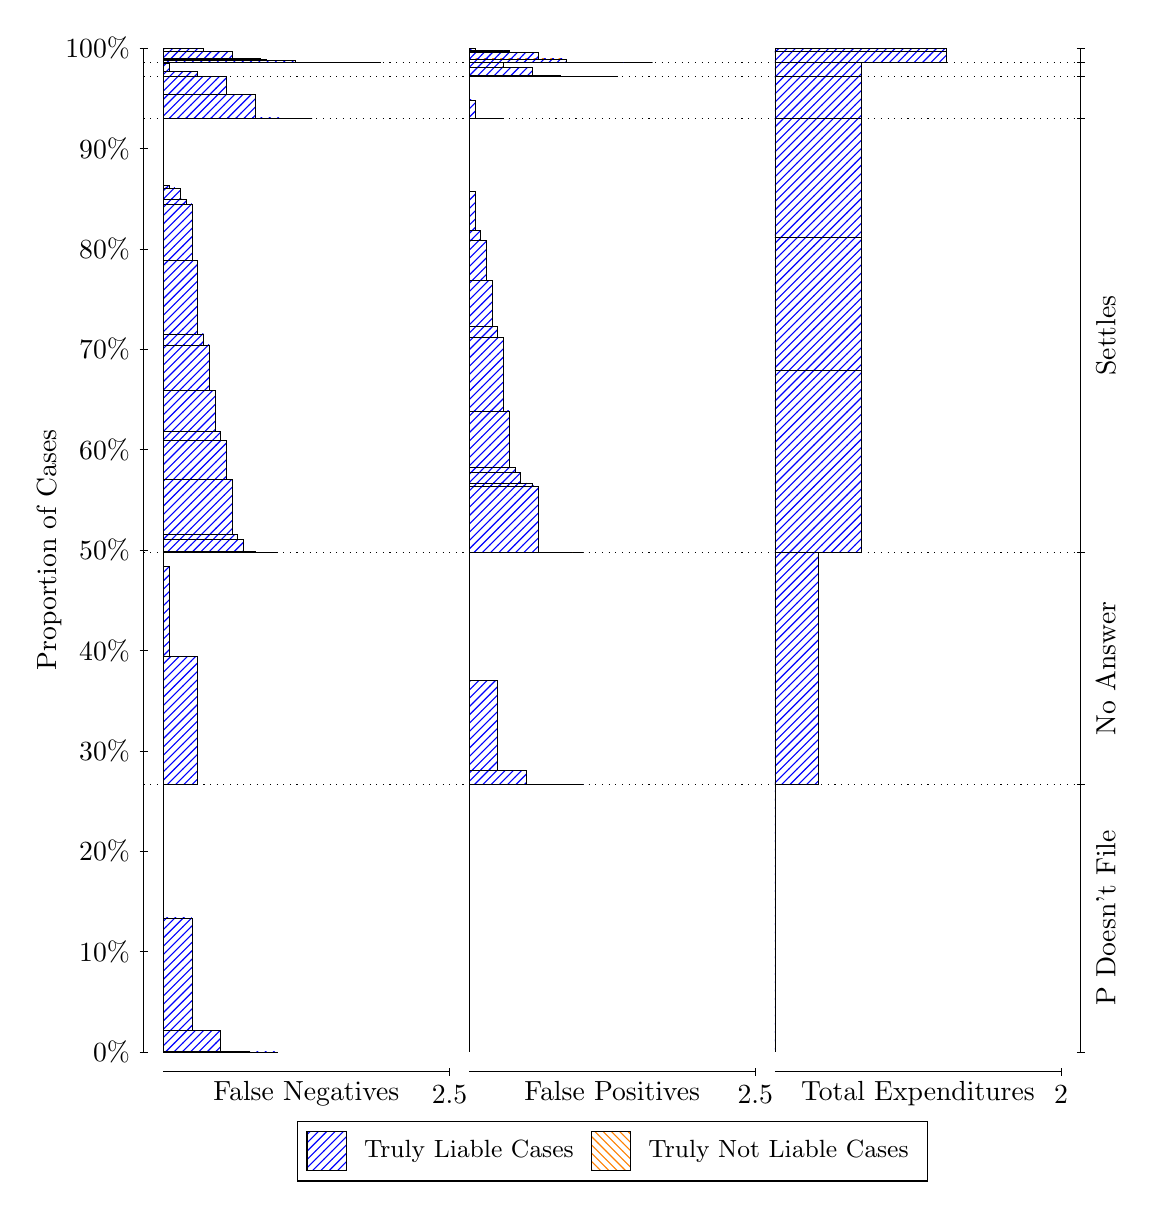
\begin{tikzpicture}
\draw[black, very thin] (1.5,1.75) -- (1.5,14.5);
\node[rotate=90, text=black, anchor=center] at (0.3, 8.125) {Proportion of Cases};
\draw[black, very thin] (1.45,1.75) -- (1.55,1.75);
\node[text=black, anchor=east] at (1.45, 1.75) {0\%};
\draw[black, very thin] (1.45,3.025) -- (1.55,3.025);
\node[text=black, anchor=east] at (1.45, 3.025) {10\%};
\draw[black, very thin] (1.45,4.3) -- (1.55,4.3);
\node[text=black, anchor=east] at (1.45, 4.3) {20\%};
\draw[black, very thin] (1.45,5.575) -- (1.55,5.575);
\node[text=black, anchor=east] at (1.45, 5.575) {30\%};
\draw[black, very thin] (1.45,6.85) -- (1.55,6.85);
\node[text=black, anchor=east] at (1.45, 6.85) {40\%};
\draw[black, very thin] (1.45,8.125) -- (1.55,8.125);
\node[text=black, anchor=east] at (1.45, 8.125) {50\%};
\draw[black, very thin] (1.45,9.4) -- (1.55,9.4);
\node[text=black, anchor=east] at (1.45, 9.4) {60\%};
\draw[black, very thin] (1.45,10.675) -- (1.55,10.675);
\node[text=black, anchor=east] at (1.45, 10.675) {70\%};
\draw[black, very thin] (1.45,11.95) -- (1.55,11.95);
\node[text=black, anchor=east] at (1.45, 11.95) {80\%};
\draw[black, very thin] (1.45,13.225) -- (1.55,13.225);
\node[text=black, anchor=east] at (1.45, 13.225) {90\%};
\draw[black, very thin] (1.45,14.5) -- (1.55,14.5);
\node[text=black, anchor=east] at (1.45, 14.5) {100\%};

\draw[black, very thin] (13.4,1.75) -- (13.4,14.5);
\draw[black, very thin] (13.35,1.75) -- (13.45,1.75);
\node[anchor=west] at (13.35, 1.75) {};
\draw[black, very thin] (13.35,5.1509) -- (13.45,5.1509);
\node[anchor=west] at (13.35, 5.1509) {};
\draw[black, very thin] (13.35,8.0904) -- (13.45,8.0904);
\node[anchor=west] at (13.35, 8.0904) {};
\draw[black, very thin] (13.35,13.608) -- (13.45,13.608);
\node[anchor=west] at (13.35, 13.608) {};
\draw[black, very thin] (13.35,14.142) -- (13.45,14.142);
\node[anchor=west] at (13.35, 14.142) {};
\draw[black, very thin] (13.35,14.317) -- (13.45,14.317);
\node[anchor=west] at (13.35, 14.317) {};
\draw[black, very thin] (13.35,14.5) -- (13.45,14.5);
\node[anchor=west] at (13.35, 14.5) {};

\draw[black, very thin, pattern color=blue, pattern=north east lines] (1.75,1.75) rectangle (3.2033,1.75);
\draw[black, very thin, pattern color=blue, pattern=north east lines] (1.75,1.75) rectangle (2.84,1.7526);
\draw[black, very thin, pattern color=blue, pattern=north east lines] (1.75,1.7526) rectangle (2.4767,2.0234);
\draw[black, very thin, pattern color=blue, pattern=north east lines] (1.75,2.0234) rectangle (2.1133,3.4536);
\draw[black, very thin, pattern color=orange, pattern=north west lines] (1.75,3.4536) rectangle (1.75,3.4536);
\draw[black, very thin, pattern color=blue, pattern=north east lines] (1.75,3.4536) rectangle (1.75,5.1509);
\draw[black, very thin, pattern color=blue, pattern=north east lines] (1.75,5.1509) rectangle (2.186,6.771);
\draw[black, very thin, pattern color=blue, pattern=north east lines] (1.75,6.771) rectangle (1.8227,7.9174);
\draw[black, very thin, pattern color=orange, pattern=north west lines] (1.75,7.9174) rectangle (1.75,7.9174);
\draw[black, very thin, pattern color=blue, pattern=north east lines] (1.75,7.9174) rectangle (1.75,8.0904);
\draw[black, very thin, pattern color=blue, pattern=north east lines] (1.75,8.0904) rectangle (3.2033,8.0904);
\draw[black, very thin, pattern color=blue, pattern=north east lines] (1.75,8.0904) rectangle (3.058,8.0905);
\draw[black, very thin, pattern color=blue, pattern=north east lines] (1.75,8.0905) rectangle (2.9127,8.1046);
\draw[black, very thin, pattern color=blue, pattern=north east lines] (1.75,8.1046) rectangle (2.84,8.1051);
\draw[black, very thin, pattern color=blue, pattern=north east lines] (1.75,8.1051) rectangle (2.7673,8.2558);
\draw[black, very thin, pattern color=blue, pattern=north east lines] (1.75,8.2558) rectangle (2.6947,8.3237);
\draw[black, very thin, pattern color=blue, pattern=north east lines] (1.75,8.3237) rectangle (2.622,9.021);
\draw[black, very thin, pattern color=blue, pattern=north east lines] (1.75,9.021) rectangle (2.5493,9.5163);
\draw[black, very thin, pattern color=blue, pattern=north east lines] (1.75,9.5163) rectangle (2.4767,9.6363);
\draw[black, very thin, pattern color=blue, pattern=north east lines] (1.75,9.6363) rectangle (2.404,10.152);
\draw[black, very thin, pattern color=blue, pattern=north east lines] (1.75,10.152) rectangle (2.3313,10.729);
\draw[black, very thin, pattern color=blue, pattern=north east lines] (1.75,10.729) rectangle (2.2587,10.869);
\draw[black, very thin, pattern color=blue, pattern=north east lines] (1.75,10.869) rectangle (2.186,11.807);
\draw[black, very thin, pattern color=blue, pattern=north east lines] (1.75,11.807) rectangle (2.1133,12.521);
\draw[black, very thin, pattern color=blue, pattern=north east lines] (1.75,12.521) rectangle (2.0407,12.585);
\draw[black, very thin, pattern color=blue, pattern=north east lines] (1.75,12.585) rectangle (1.968,12.721);
\draw[black, very thin, pattern color=blue, pattern=north east lines] (1.75,12.721) rectangle (1.8953,12.723);
\draw[black, very thin, pattern color=blue, pattern=north east lines] (1.75,12.723) rectangle (1.8227,12.758);
\draw[black, very thin, pattern color=orange, pattern=north west lines] (1.75,12.758) rectangle (1.75,12.758);
\draw[black, very thin, pattern color=blue, pattern=north east lines] (1.75,12.758) rectangle (1.75,13.608);
\draw[black, very thin, pattern color=blue, pattern=north east lines] (1.75,13.608) rectangle (3.6393,13.608);
\draw[black, very thin, pattern color=blue, pattern=north east lines] (1.75,13.608) rectangle (3.276,13.614);
\draw[black, very thin, pattern color=blue, pattern=north east lines] (1.75,13.614) rectangle (2.9127,13.909);
\draw[black, very thin, pattern color=blue, pattern=north east lines] (1.75,13.909) rectangle (2.5493,14.139);
\draw[black, very thin, pattern color=blue, pattern=north east lines] (1.75,14.139) rectangle (2.186,14.142);
\draw[black, very thin, pattern color=orange, pattern=north west lines] (1.75,14.142) rectangle (1.75,14.142);
\draw[black, very thin, pattern color=blue, pattern=north east lines] (1.75,14.142) rectangle (2.186,14.208);
\draw[black, very thin, pattern color=blue, pattern=north east lines] (1.75,14.208) rectangle (1.8227,14.308);
\draw[black, very thin, pattern color=orange, pattern=north west lines] (1.75,14.308) rectangle (1.75,14.308);
\draw[black, very thin, pattern color=blue, pattern=north east lines] (1.75,14.308) rectangle (1.75,14.317);
\draw[black, very thin, pattern color=blue, pattern=north east lines] (1.75,14.317) rectangle (4.5113,14.317);
\draw[black, very thin, pattern color=blue, pattern=north east lines] (1.75,14.317) rectangle (4.148,14.317);
\draw[black, very thin, pattern color=blue, pattern=north east lines] (1.75,14.317) rectangle (3.7847,14.321);
\draw[black, very thin, pattern color=blue, pattern=north east lines] (1.75,14.321) rectangle (3.712,14.321);
\draw[black, very thin, pattern color=blue, pattern=north east lines] (1.75,14.321) rectangle (3.4213,14.345);
\draw[black, very thin, pattern color=blue, pattern=north east lines] (1.75,14.345) rectangle (3.3487,14.345);
\draw[black, very thin, pattern color=blue, pattern=north east lines] (1.75,14.345) rectangle (3.058,14.351);
\draw[black, very thin, pattern color=blue, pattern=north east lines] (1.75,14.351) rectangle (2.9853,14.37);
\draw[black, very thin, pattern color=blue, pattern=north east lines] (1.75,14.37) rectangle (2.6947,14.37);
\draw[black, very thin, pattern color=blue, pattern=north east lines] (1.75,14.37) rectangle (2.622,14.456);
\draw[black, very thin, pattern color=blue, pattern=north east lines] (1.75,14.456) rectangle (2.3313,14.456);
\draw[black, very thin, pattern color=blue, pattern=north east lines] (1.75,14.456) rectangle (2.2587,14.498);
\draw[black, very thin, pattern color=blue, pattern=north east lines] (1.75,14.498) rectangle (1.8953,14.5);
\draw[black, very thin, pattern color=orange, pattern=north west lines] (1.75,14.5) rectangle (1.75,14.5);
\draw[black, very thin, pattern color=blue, pattern=north east lines] (1.75,14.5) rectangle (1.75,14.5);
\draw[black, very thin, pattern color=orange, pattern=north west lines] (5.6333,1.75) rectangle (5.6333,1.75);
\draw[black, very thin, pattern color=blue, pattern=north east lines] (5.6333,1.75) rectangle (5.6333,5.1509);
\draw[black, very thin, pattern color=orange, pattern=north west lines] (5.6333,5.1509) rectangle (7.0867,5.1509);
\draw[black, very thin, pattern color=blue, pattern=north east lines] (5.6333,5.1509) rectangle (7.0867,5.1509);
\draw[black, very thin, pattern color=blue, pattern=north east lines] (5.6333,5.1509) rectangle (6.7233,5.1512);
\draw[black, very thin, pattern color=blue, pattern=north east lines] (5.6333,5.1512) rectangle (6.36,5.3239);
\draw[black, very thin, pattern color=blue, pattern=north east lines] (5.6333,5.3239) rectangle (5.9967,6.4703);
\draw[black, very thin, pattern color=blue, pattern=north east lines] (5.6333,6.4703) rectangle (5.6333,8.0904);
\draw[black, very thin, pattern color=orange, pattern=north west lines] (5.6333,8.0904) rectangle (7.0867,8.0904);
\draw[black, very thin, pattern color=blue, pattern=north east lines] (5.6333,8.0904) rectangle (7.0867,8.0904);
\draw[black, very thin, pattern color=orange, pattern=north west lines] (5.6333,8.0904) rectangle (6.9413,8.0904);
\draw[black, very thin, pattern color=blue, pattern=north east lines] (5.6333,8.0904) rectangle (6.9413,8.0904);
\draw[black, very thin, pattern color=orange, pattern=north west lines] (5.6333,8.0904) rectangle (6.796,8.0904);
\draw[black, very thin, pattern color=blue, pattern=north east lines] (5.6333,8.0904) rectangle (6.796,8.0904);
\draw[black, very thin, pattern color=blue, pattern=north east lines] (5.6333,8.0904) rectangle (6.7233,8.0904);
\draw[black, very thin, pattern color=orange, pattern=north west lines] (5.6333,8.0904) rectangle (6.6507,8.0904);
\draw[black, very thin, pattern color=blue, pattern=north east lines] (5.6333,8.0904) rectangle (6.6507,8.0917);
\draw[black, very thin, pattern color=blue, pattern=north east lines] (5.6333,8.0917) rectangle (6.578,8.0918);
\draw[black, very thin, pattern color=orange, pattern=north west lines] (5.6333,8.0918) rectangle (6.5053,8.0918);
\draw[black, very thin, pattern color=blue, pattern=north east lines] (5.6333,8.0918) rectangle (6.5053,8.9405);
\draw[black, very thin, pattern color=blue, pattern=north east lines] (5.6333,8.9405) rectangle (6.4327,8.9755);
\draw[black, very thin, pattern color=blue, pattern=north east lines] (5.6333,8.9755) rectangle (6.36,8.9769);
\draw[black, very thin, pattern color=blue, pattern=north east lines] (5.6333,8.9769) rectangle (6.2873,9.113);
\draw[black, very thin, pattern color=blue, pattern=north east lines] (5.6333,9.113) rectangle (6.2147,9.1767);
\draw[black, very thin, pattern color=blue, pattern=north east lines] (5.6333,9.1767) rectangle (6.142,9.8915);
\draw[black, very thin, pattern color=blue, pattern=north east lines] (5.6333,9.8915) rectangle (6.0693,10.829);
\draw[black, very thin, pattern color=blue, pattern=north east lines] (5.6333,10.829) rectangle (5.9967,10.969);
\draw[black, very thin, pattern color=blue, pattern=north east lines] (5.6333,10.969) rectangle (5.924,11.546);
\draw[black, very thin, pattern color=blue, pattern=north east lines] (5.6333,11.546) rectangle (5.8513,12.062);
\draw[black, very thin, pattern color=blue, pattern=north east lines] (5.6333,12.062) rectangle (5.7787,12.182);
\draw[black, very thin, pattern color=blue, pattern=north east lines] (5.6333,12.182) rectangle (5.706,12.677);
\draw[black, very thin, pattern color=blue, pattern=north east lines] (5.6333,12.677) rectangle (5.6333,13.608);
\draw[black, very thin, pattern color=orange, pattern=north west lines] (5.6333,13.608) rectangle (6.0693,13.608);
\draw[black, very thin, pattern color=blue, pattern=north east lines] (5.6333,13.608) rectangle (6.0693,13.61);
\draw[black, very thin, pattern color=blue, pattern=north east lines] (5.6333,13.61) rectangle (5.706,13.841);
\draw[black, very thin, pattern color=blue, pattern=north east lines] (5.6333,13.841) rectangle (5.6333,14.142);
\draw[black, very thin, pattern color=orange, pattern=north west lines] (5.6333,14.142) rectangle (7.5227,14.142);
\draw[black, very thin, pattern color=blue, pattern=north east lines] (5.6333,14.142) rectangle (7.5227,14.142);
\draw[black, very thin, pattern color=blue, pattern=north east lines] (5.6333,14.142) rectangle (7.1593,14.142);
\draw[black, very thin, pattern color=blue, pattern=north east lines] (5.6333,14.142) rectangle (6.796,14.151);
\draw[black, very thin, pattern color=blue, pattern=north east lines] (5.6333,14.151) rectangle (6.4327,14.251);
\draw[black, very thin, pattern color=blue, pattern=north east lines] (5.6333,14.251) rectangle (6.0693,14.317);
\draw[black, very thin, pattern color=orange, pattern=north west lines] (5.6333,14.317) rectangle (7.9587,14.317);
\draw[black, very thin, pattern color=blue, pattern=north east lines] (5.6333,14.317) rectangle (7.9587,14.317);
\draw[black, very thin, pattern color=orange, pattern=north west lines] (5.6333,14.317) rectangle (7.5953,14.317);
\draw[black, very thin, pattern color=blue, pattern=north east lines] (5.6333,14.317) rectangle (7.5953,14.317);
\draw[black, very thin, pattern color=orange, pattern=north west lines] (5.6333,14.317) rectangle (7.232,14.317);
\draw[black, very thin, pattern color=blue, pattern=north east lines] (5.6333,14.317) rectangle (7.232,14.319);
\draw[black, very thin, pattern color=blue, pattern=north east lines] (5.6333,14.319) rectangle (6.8687,14.361);
\draw[black, very thin, pattern color=orange, pattern=north west lines] (5.6333,14.361) rectangle (6.8687,14.361);
\draw[black, very thin, pattern color=blue, pattern=north east lines] (5.6333,14.361) rectangle (6.8687,14.361);
\draw[black, very thin, pattern color=orange, pattern=north west lines] (5.6333,14.361) rectangle (6.796,14.361);
\draw[black, very thin, pattern color=blue, pattern=north east lines] (5.6333,14.361) rectangle (6.796,14.361);
\draw[black, very thin, pattern color=blue, pattern=north east lines] (5.6333,14.361) rectangle (6.5053,14.446);
\draw[black, very thin, pattern color=blue, pattern=north east lines] (5.6333,14.446) rectangle (6.5053,14.447);
\draw[black, very thin, pattern color=orange, pattern=north west lines] (5.6333,14.447) rectangle (6.4327,14.447);
\draw[black, very thin, pattern color=blue, pattern=north east lines] (5.6333,14.447) rectangle (6.4327,14.447);
\draw[black, very thin, pattern color=blue, pattern=north east lines] (5.6333,14.447) rectangle (6.142,14.456);
\draw[black, very thin, pattern color=blue, pattern=north east lines] (5.6333,14.456) rectangle (6.142,14.466);
\draw[black, very thin, pattern color=blue, pattern=north east lines] (5.6333,14.466) rectangle (6.0693,14.472);
\draw[black, very thin, pattern color=orange, pattern=north west lines] (5.6333,14.472) rectangle (6.0693,14.472);
\draw[black, very thin, pattern color=blue, pattern=north east lines] (5.6333,14.472) rectangle (6.0693,14.472);
\draw[black, very thin, pattern color=blue, pattern=north east lines] (5.6333,14.472) rectangle (5.7787,14.472);
\draw[black, very thin, pattern color=blue, pattern=north east lines] (5.6333,14.472) rectangle (5.7787,14.472);
\draw[black, very thin, pattern color=blue, pattern=north east lines] (5.6333,14.472) rectangle (5.706,14.495);
\draw[black, very thin, pattern color=blue, pattern=north east lines] (5.6333,14.495) rectangle (5.706,14.496);
\draw[black, very thin, pattern color=blue, pattern=north east lines] (5.6333,14.496) rectangle (5.6333,14.5);
\draw[black, very thin, pattern color=orange, pattern=north west lines] (9.5167,1.75) rectangle (9.5167,1.75);
\draw[black, very thin, pattern color=blue, pattern=north east lines] (9.5167,1.75) rectangle (9.5167,5.1509);
\draw[black, very thin, pattern color=orange, pattern=north west lines] (9.5167,5.1509) rectangle (10.062,5.1509);
\draw[black, very thin, pattern color=blue, pattern=north east lines] (9.5167,5.1509) rectangle (10.062,8.0904);
\draw[black, very thin, pattern color=orange, pattern=north west lines] (9.5167,8.0904) rectangle (10.607,8.0904);
\draw[black, very thin, pattern color=blue, pattern=north east lines] (9.5167,8.0904) rectangle (10.607,10.411);
\draw[black, very thin, pattern color=orange, pattern=north west lines] (9.5167,10.411) rectangle (10.607,10.411);
\draw[black, very thin, pattern color=blue, pattern=north east lines] (9.5167,10.411) rectangle (10.607,12.095);
\draw[black, very thin, pattern color=orange, pattern=north west lines] (9.5167,12.095) rectangle (10.607,12.095);
\draw[black, very thin, pattern color=blue, pattern=north east lines] (9.5167,12.095) rectangle (10.607,13.608);
\draw[black, very thin, pattern color=orange, pattern=north west lines] (9.5167,13.608) rectangle (10.607,13.608);
\draw[black, very thin, pattern color=blue, pattern=north east lines] (9.5167,13.608) rectangle (10.607,14.142);
\draw[black, very thin, pattern color=orange, pattern=north west lines] (9.5167,14.142) rectangle (10.607,14.142);
\draw[black, very thin, pattern color=blue, pattern=north east lines] (9.5167,14.142) rectangle (10.607,14.317);
\draw[black, very thin, pattern color=orange, pattern=north west lines] (9.5167,14.317) rectangle (11.697,14.317);
\draw[black, very thin, pattern color=blue, pattern=north east lines] (9.5167,14.317) rectangle (11.697,14.455);
\draw[black, very thin, pattern color=orange, pattern=north west lines] (9.5167,14.455) rectangle (11.697,14.455);
\draw[black, very thin, pattern color=blue, pattern=north east lines] (9.5167,14.455) rectangle (11.697,14.5);
\draw[black, dotted] (1.5,5.1509) -- (13.4,5.1509);
\draw[black, dotted] (1.5,8.0904) -- (13.4,8.0904);
\draw[black, dotted] (1.5,13.608) -- (13.4,13.608);
\draw[black, dotted] (1.5,14.142) -- (13.4,14.142);
\draw[black, dotted] (1.5,14.317) -- (13.4,14.317);
\draw[black, very thin] (1.75,1.5) -- (5.3833,1.5);
\node[text=black, anchor=north] at (3.5667, 1.5) {False Negatives};
\draw[black, very thin] (5.3833,1.45) -- (5.3833,1.55);
\node[text=black, anchor=north] at (5.3833, 1.45) {2.5};

\draw[black, very thin] (5.6333,1.5) -- (9.2667,1.5);
\node[text=black, anchor=north] at (7.45, 1.5) {False Positives};
\draw[black, very thin] (9.2667,1.45) -- (9.2667,1.55);
\node[text=black, anchor=north] at (9.2667, 1.45) {2.5};

\draw[black, very thin] (9.5167,1.5) -- (13.15,1.5);
\node[text=black, anchor=north] at (11.333, 1.5) {Total Expenditures};
\draw[black, very thin] (13.15,1.45) -- (13.15,1.55);
\node[text=black, anchor=north] at (13.15, 1.45) {2};

\node[text=black, centered, rotate=90] at (13.72, 3.4504) {P Doesn't File};
\node[text=black, centered, rotate=90] at (13.72, 6.6206) {No Answer};
\node[text=black, centered, rotate=90] at (13.72, 10.849) {Settles};




\draw (7.449999999999999,1.5) node[draw=none] (baseCoordinate) {};
\begin{scope}[align=center]
        \matrix[scale=0.5, draw=black, below=0.5cm of baseCoordinate, nodes={draw}, column sep=0.1cm]{
            \node[rectangle, draw, minimum width=0.5cm, minimum height=0.5cm, pattern color=blue, pattern=north east lines] {}; &
            \node[draw=none, font=\small, text=black] (B) {Truly Liable Cases}; &
            \node[rectangle, draw, minimum width=0.5cm, minimum height=0.5cm, pattern color=orange, pattern=north west lines] {}; &
            \node[draw=none, font=\small, text=black] (B) {Truly Not Liable Cases}; \\
            };
\end{scope}

\end{tikzpicture}
\end{document}